\chapter{Method}\label{chap:method}
% big overview with a graph
\begin{figure}[h]
	\centering
	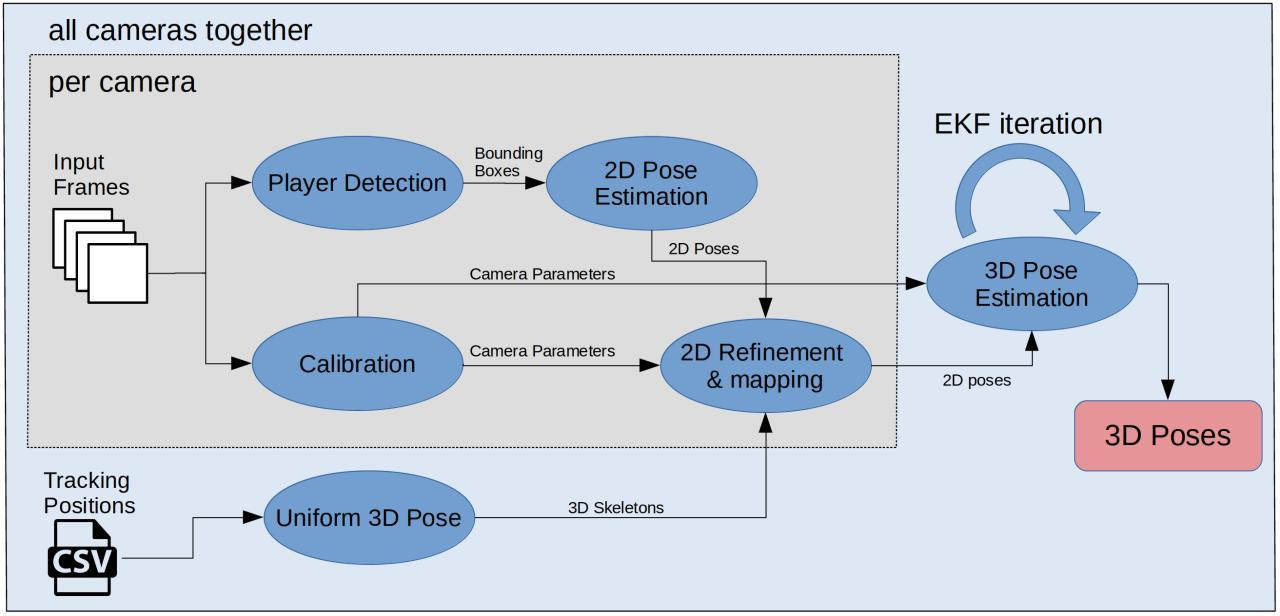
\includegraphics[width=1.0\textwidth]{./images/overview.jpg}
	\caption{Overview of the workflow. Each step gets described in detail during this chapter. The gray area is the process for each camera separately while in the blue area the different cameras are merged.}
	\label{fig:overview}
\end{figure}

\section{Calibration}\label{sec:calibration}
% what is used from soccer on tabletop
In order to work in three-dimensional space it is required to know how the pixels in a two-dimensional image relate to the three-dimensional world. For the camera model we consider the pinhole camera model for simplicity despite the fact that some cameras suffer from distortion. As mentioned in section \ref{tablecalibration} we were able to calibrate the cameras and got the corresponding camera matrix $M$ which transforms homogeneous 3D world coordinates to homogeneous 2D image coordinates. 

\subsection{Camera Matrix}\label{sec:cameramatrix}
% informations from http://ksimek.github.io/2012/08/14/decompose/

\subsection{Line Detection}
% maybe some details about it

\section{Player Detection}
% details about Detectron

\section{2D Pose Estimation}\label{sec:poseestimation}
% details about openpose

\section{2D Refinement \& mapping}\label{sec:2drefinement}
% details about openpose

\section{3D Pose Estimation}
Now I have to determine the points in 3D space given its projections onto the multiple images from the different camera perspectives. By knowing the camera matrix of the camera projection from 3D to 2D we know that each point in the image corresponds to a line in 3D space and every point on this line get projected on the same point in the 2D image as mentioned in section \ref{sec:calibration}.

\subsection{Triangulation}
The method to solve this problem is called triangulation. In theory with perfect measurements this method is trivial. So let's assume we got a pair $y_1$ and $y_2$ of corresponding points in two different images. Remember that each point in the image belongs to a line in 3D space which are the green lines in the figure \ref{fig:triangulation} below. The lines intersect at $x$ which is the corresponding point in 3D space. 
\begin{figure}[h]
	\centering
	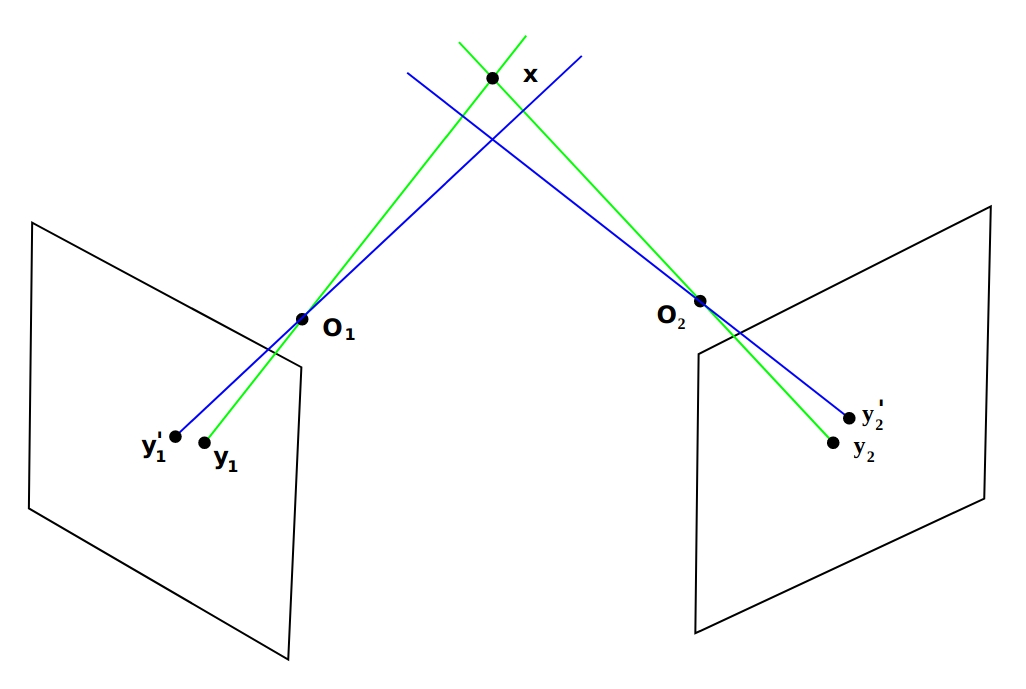
\includegraphics[width=0.6\textwidth]{./images/TriangulationReal.jpg}
	\captionsource{Triangulation visualization of two images with the camera's focal length $O_1$ and $O_2$. The ideal case with perfect measurements in green and the case of measurements with arbitrary accuracy in blue.}{\cite{triangulation}}
	\label{fig:triangulation}
\end{figure}\\
But in practice the the image points are measured with arbitrary accuracy. This leads to the two points $y_1'$ and $y_2'$ in the figure \ref{fig:triangulation}. If you consider the corresponding lines of these two points in 3D space (blue), they must not even intersect and if they do it's not correctly the expected point $x$. Reasons for the deviations may be noisy measurements or an inaccurate camera calibration which lead to wrong focal lengths $O_1$ and $O_2$ and therefore to a wrong projection. \\

To find out which 3D point $x'$  is the best estimate for the noisy measurements $y_1'$ and $y_2'$ you usually define an error measurement depending on $x'$ and then minimize this error. Due to the fact that I don't always get all poses in 2D for the triangulation and the camera calibration is not error-free, I tried to use the Kalman Filter to do the triangulation. By constantly getting new measurements over time and the possibility of predicting the state further in time it seems to be a suitable application. 


\subsection{Extended Kalman Filter}\label{sec:EKF}
% details about EKF
The Kalman Filter (KF) is an iterative algorithm, based on the Bayesian Filter, that uses a series of measurements observed over time to find a good state estimation \cite{filterpybook}. The filter estimates the state using a form of feedback control where the measured values come into play.

\begin{figure}[h]
	\centering
	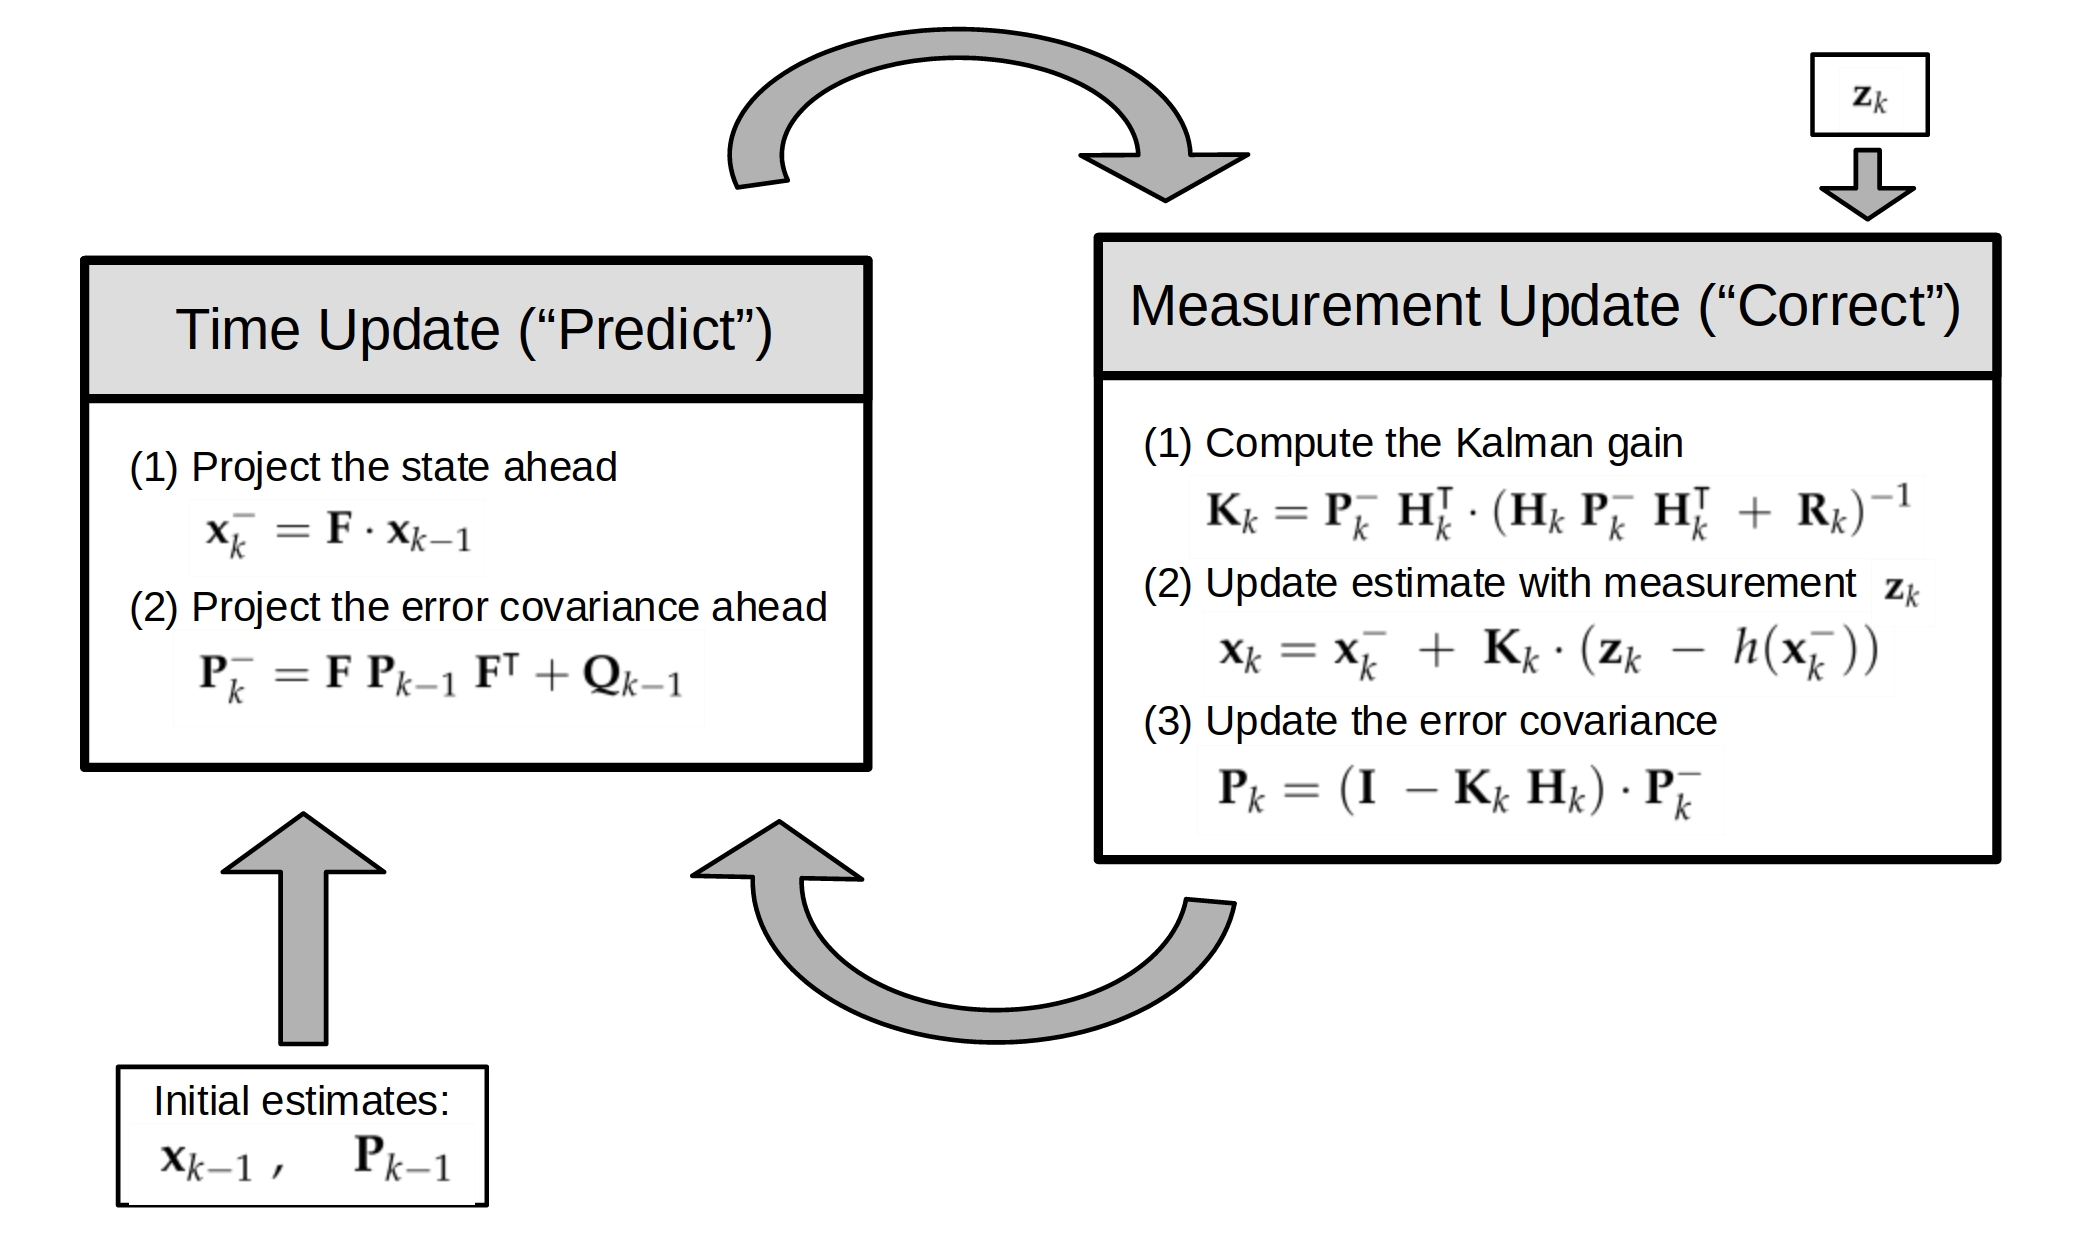
\includegraphics[width=1.0\textwidth]{./images/kalman.jpg}
	\captionsource{Complete picture of the calculations during the two-step process of the Extended Kalman Filter. For the Initialization the values of the first state vector and the error covariance are needed. A new measurement vector is given to the filter for each Measurement Update step. }{Notation slightly adapted from \cite{kalmanbook}}
	\label{fig:kalmanprocess}
\end{figure}
The algorithm works in a two-step process as shown below in figure \ref{fig:kalmanprocess} which is repeated for every time step which is in my case the next frame. In the prediction step, the Kalman Filter projects the current state variable forward in time using the process model and projects the error covariance ahead. In the second step, called the update step, the previously estimated state variable gets updated using the measurement residual weighted with the so called Kalman gain. Additionally the error covariance is updated.
and a new external measurement as described in section x.

To update the state variable the measurement residual is needed which is computed using the current state variable and a new measurement $\mathbf{z}_k$ as described in section \ref{sec:2drefinement}. But the state variable is not part of the measurement space, therefore we have to project the state variable to the measurement space. This projection is basically a camera projection and is not linear due to a division, which is the reason why I use the Extended Kalman Filter (EKF). The reason why I work in measurement space and not in state space is because the measurements are not simply invertible.  

\subsection{Designing the EKF} 
In the figure \ref{fig:kalmanprocess} and in the following text I will use the notation from the book \textit{An Introduction to the Kalman Filter} \cite{kalmanbook} slightly adapted to the filterpy \cite{filterpybook} notation. I will omit the time subscript $k$ for the definitions of multiple variables in this section for the sake of clarity. For coordinates $x,y,z$ I use the subscript $w$ for the 3D space and $c_k$ for the 2D space of the $k$-th camera. The state and measurement variable $\mathbf{x}, \mathbf{z}$ are written in bold to distinguish from the $x$ and $z$ coordinates. The last note is about the camera matrices which change with every frame. So when I mention them I always refer to the current calibration.

\subsubsection{State and Measurement}
The EKF is designed to track one person using five different cameras. As mentioned in section \ref{sec:poseestimation} the OpenPose model \textit{COCO} consists of 15 keypoints. For the $i$-th keypoint the corresponding part of the state vector includes the position in 3D space and their velocities:
\begin{equation}
\mathbf{x}^i \coloneqq 
\begin{bmatrix}
x^i_{w} & y^i_{w} & z^i_{w} & v^i_{x} & v^i_{y} & v^i_{z}\\
\end{bmatrix}^\intercal,   \ \ \forall i \in \{0,1,...,17\}
\end{equation}
All 18 keypoints together form the state vector:
\begin{equation}
\mathbf{x} \coloneqq 
\begin{bmatrix}
\mathbf{x}^0 & \mathbf{x}^1 & \cdots & \mathbf{x}^{17}\\
\end{bmatrix}^\intercal
\end{equation}
The measurement vector $\mathbf{z}$ includes for the $i$-th keypoint the image coordinates $x, y$ for all five cameras:
\begin{equation}
\mathbf{z}^i \coloneqq 
\begin{bmatrix}
x^i_{c_0} & y^i_{c_0} & x^i_{c_1} & y^i_{c_1} & \cdots & x^i_{c_4} & y^i_{c_4}\\
\end{bmatrix}^\intercal, \ \ \forall i \in \{0,1,...,17\}
\end{equation}
The complete measurement vector is again for all 18 keypoints:
\begin{equation}
\mathbf{z} \coloneqq 
\begin{bmatrix}
\mathbf{z}^0 & \mathbf{z}^1 & \cdots & \mathbf{z}^{17}\\
\end{bmatrix}^\intercal
\end{equation}

\subsubsection{Process Model}
For the state propagation $\mathbf{F}$ in the Predict step I use a simple linear model that does not change over time. For the sake of simplicity i assume constant velocity. For several reasons this is not the best choice for modeling the real world. The players move in different directions, the head keypoints behave completely differently to the hand keypoints etc. But due to the high frame rate one can neglect these aspects because the movement from one frame to the next is minimal. The linear motion model for the $x$ coordinates in 3D space is as follows $x = x + v_x\cdot \Delta t$. The time step $\Delta t$ represents the time between two frames. The resulting state transition model $F'$ propagates the state vector for the $i$-th keypoint $x^i$ further in time,
\begin{equation}
\mathbf{F}^i \coloneqq 
\begin{bmatrix}
1 & 0 & 0 & \Delta t & 0 & 0 \\
0 & 1 & 0 & 0 & \Delta t & 0 \\
0 & 0 & 1 & 0 & 0 & \Delta t \\
0 & 0 & 0 & 1 & 0 & 0 \\
0 & 0 & 0 & 0 & 1 & 0 \\
0 & 0 & 0 & 0 & 0 & 1 \\
\end{bmatrix}, \ \ \forall i \in \{0,...,17\}
\end{equation}
so the resulting complete state propagation matrix $\mathbf{F}$ is a diagional matrix expressed using multiple submatrices $\mathbf{F}^i$:
\begin{equation}
\mathbf{F} \coloneqq 
\begin{bmatrix}
\mathbf{F}^1 & & \\
& \ddots & \\
& & \mathbf{F}^{17}
\end{bmatrix}
\end{equation}
This results in the first equation of our extended Kalman filter to project the state ahead:
\begin{equation}\label{eq:state}
\mathbf{x}_k^- = \mathbf{F} \cdot \mathbf{x}_{k-1}
\end{equation}

Together with the next equation \ref{eq:covariance}, those two form the prediction step of the EKF. The estimation error covariance $\mathbf{P}$ gets projected  from the previous time step $k-1$ to the current time step $k$.
\begin{equation}\label{eq:covariance}
\mathbf{P}_k^- = \mathbf{F}\ \mathbf{P}_{k-1}\ \mathbf{F}^\intercal + \mathbf{Q}_{k-1}
\end{equation}
To start you have to initialize the covariance matrix $\mathbf{P}$ and then the filter takes care of updating its value. We know that the position and velocity are correlated but due to the fact that we use constant velocity in our model we just initialize $\mathbf{P}$ to zero. The matrix is a square matrix of the same dimension as the state vector. 

\subsubsection{Noise}
In both equation \ref{eq:covariance} and \ref{eq:covariance2} we add a covariance matrix derived from white Gaussian noise. $\mathbf{Q}$ is a square matrix of the same dimension as the state vector $\mathbf{x}_k$ and is called the process noise covariance. The matrix $\mathbf{R}$ is also a square matrix with the dimension of the measurement vector $\mathbf{z}_k$ and is called the measurement noise covariance. They're called white Gaussian noise because they are independent of each other with normal probability distribution. During the EKF iteration they stay constant with values $\sigma_q = 0.3$ and $\sigma_r = 0.02$:
\begin{equation}
	\mathbf{Q} \coloneqq 
	\begin{bmatrix}
	\sigma_q & & \\
	& \ddots & \\
	& & \sigma_q
	\end{bmatrix}
\ \qquad \qquad \qquad \qquad 
\mathbf{R} \coloneqq 
\begin{bmatrix}
\sigma_r & & \\
& \ddots & \\
& & \sigma_r
\end{bmatrix}
\end{equation}
The reason for the higher process noise is the inaccurate process model with constant velocity. So the filter tries to rely more on the measurements than on the prediction.


\subsubsection{Kalman gain and Error covariance}
The residual gets added to the predicted state variable $\mathbf{x}_k^-$ as described in the section below. But the residual is weighted by the Kalman gain. Higher values for the Kalman gain indicate that we give more trust to the measurement and a lower values indicate that we rely more on the prediction. So if the measurement uncertainty $\mathbf{R}_k$ is smaller with respect to the error covariance $\mathbf{P}_k^-$ we rely more on the measurement. The computation for the Kalman gain takes place in the Measurement Update step: 
\begin{equation}
\mathbf{K}_k = \mathbf{P}_k^-\ \mathbf{H}_k^\intercal\cdot (\mathbf{H}_k\ \mathbf{P}_k^-\ \mathbf{H}_k^\intercal \ + \ \mathbf{R}_k)^{-1}
\end{equation}
Another equation in the Measurement Update step is the update of the error covariance $\mathbf{P}_k$. 
\begin{equation}\label{eq:covariance2}
\mathbf{P}_k = (\mathbf{I} \ - \mathbf{K}_k\ \mathbf{H}_k)\cdot \mathbf{P}_k^-
\end{equation}
In contrast to $\mathbf{Q}$ and $\mathbf{R}$ which are both constant, the error covariance $\mathbf{P}_k$ and the Kalman gain $\mathbf{K}_k$ will stabilize quickly and then remain constant as described in \cite{kalmanbook}.
These two equations involves the matrix $\mathbf{H}$ which is explained in the section \ref{sec:jacobian} below.

\subsubsection{Measurement Model}
The measurement model is designed through a function $h$ which is responsible to relate the state vector $\mathbf{x}_k$ to the measurement $\mathbf{z}_k$. As I mentioned in section \ref{sec:EKF} this function projects the state variable into the measurement space in order to be able to compute the residual which leads to this equation for the Measurement Update step:
\begin{equation}
\mathbf{x}_k = \mathbf{x}_k^- \ + \ \mathbf{K}_k\cdot (\mathbf{z}_k \ - \ h(\mathbf{x}_k^-))
\end{equation}
I will explain right  away in detail how the function $h$ looks like and what the related matrix $\mathbf{H}_x$ is. The filterpy implementation \cite{filterpydoc} of the EKF requires for the update step the function $h$ with the arguments $\mathbf{x}_k$ and the camera matrices for all five cameras. The output of this function is a vector which looks exactly like the measurement vector $\mathbf{z}_k$ but don't get confused, it's just the same space and no new measurement vector:
\begin{equation}
h(\mathbf{x}^-_k, \text{camera matrices}) = \mathbf{z}_{transformed}
\end{equation}

As mentioned in section \ref{sec:cameramatrix} a homogeneous point in the 3D space can be projected to the image screen using the camera matrix $\mathbf{M}$. I will explain this step for the $x_w,y_w,z_w$ coordinates of the state vector $\mathbf{x}_k$ for one keypoint to map to the corresponding measurement space of one specific camera $j$. I will omit the time subscript $k$ in this section for the sake of understanding. 
\begin{align} 
\mathbf{M}_{c_j} \cdot 
\begin{bmatrix}
x_w \\
y_w \\
z_w \\
1 \\
\end{bmatrix} &= 
\mathbf{A}_{c_j} \begin{bmatrix}
\mathbf{R}_{c_j}&|&\mathbf{T}_{c_j} \\
\end{bmatrix}
\begin{bmatrix}
x_w \\
y_w \\
z_w \\
1 \\
\end{bmatrix} \\
& = 
\begin{bmatrix}
f_x & 0 & x_0 \\
0 & f_y & y_0 \\
0 & 0 & 1\\
\end{bmatrix} 
\begin{bmatrix}
r_{1,1} & r_{1,2} & r_{1,3}& t_x \\
r_{2,1} & r_{2,2} & r_{2,3}& t_y \\
r_{3,1} & r_{3,2} & r_{3,3}& t_z \\
\end{bmatrix}
\begin{bmatrix}
x_w \\
y_w \\
z_w \\
1 \\
\end{bmatrix} \\
& = 
\begin{bmatrix}\label{eq:homogenous}
x_{c_j}' \\
y_{c_j}' \\
z_{c_j}' \\
\end{bmatrix}
\end{align}
In order to get the correct scale and dimension for the screen coordinates  $x_{c_j}, y_{c_j}$ one have to divide the result from equation \ref{eq:homogenous} by $z_{c_j}$ and drop the last entry for the $z$ coordinate. This forms a part of the function $h$:
\begin{align}\label{eq:screencoordinates}
\hat{h}(\begin{bmatrix}
x_w \\
y_w \\
z_w \\
\end{bmatrix},\  \mathbf{A}_{c_j}, \mathbf{R}_{c_j}, \mathbf{T}_{c_j}) &=
\begin{bmatrix}
	x_{c_j} \\
	y_{c_j} \\
\end{bmatrix} \\
&= 
\begin{bmatrix}
\frac{x_{c_j}'}{z_{c_j}'} \\
\frac{y_{c_j}'}{z_{c_j}'} \\
\end{bmatrix} = 
\begin{bmatrix}
\frac{f_x \cdot (r_{1,1} \cdot x_w + r_{1,2} \cdot y_w + r_{1,3} \cdot z_w + t_x)}{r_{3,1} \cdot x_w + r_{3,2} \cdot y_w + r_{3,3} \cdot z_w + t_z } + x_0 \\
\frac{f_y \cdot (r_{2,1} \cdot x_w + r_{2,2} \cdot y_w + r_{2,3} \cdot z_w + t_x)}{r_{3,1} \cdot x_w + r_{3,2} \cdot y_w + r_{3,3} \cdot z_w + t_z } + y_0 \\
\end{bmatrix}
\end{align}
To make it clear once again, this was just to transform the 3D coordinates for one keypoint into the image space of one camera. So for the $i$-th keypoint of the state vector $\mathbf{x}_k$ we drop the velocities and transform the 3D coordinates to screen coordinates for each camera. This gives us a bigger part of $h$:
\begin{align}
h_i(\begin{bmatrix}
x^i_w \\
y^i_w \\
z^i_w \\
\end{bmatrix},\ \text{camera matrices}) 
& = 
\begin{bmatrix}
\hat{h}(
\begin{bmatrix}
x^i_w \\
y^i_w \\
z^i_w \\
\end{bmatrix},\  \mathbf{A}_{c_0}, \mathbf{R}_{c_0}, \mathbf{T}_{c_0})\\
\vdots \\
\hat{h}(
\begin{bmatrix}
x^i_w \\
y^i_w \\
z^i_w \\
\end{bmatrix},\  \mathbf{A}_{c_4}, \mathbf{R}_{c_4}, \mathbf{T}_{c_4})
\end{bmatrix}
\end{align}
Finally we can formulate the whole function $h$:
\begin{align}
h(\mathbf{x}^-_k, \text{camera matrices}) 
&= 
\begin{bmatrix}
h_0(\begin{bmatrix}
x^0_w \\
y^0_w \\
z^0_w \\
\end{bmatrix},\ \text{camera matrices})\\
\vdots \\
h_{17}(\begin{bmatrix}
x^{17}_w \\
y^{17}_w \\
z^{17}_w \\
\end{bmatrix},\ \text{camera matrices}) 
\end{bmatrix}\\
&= \mathbf{z}_{transformed}
\end{align}

\subsubsection{Jacobian Matrix H} \label{sec:jacobian}
By the fact that the relationship between state space and the measurement space is a nonlinear function $h$ we need to linearize it by evaluating its partial derivatives with respect to the state vector $\mathbf{x}_k$ like a Taylor series. The resulting matrix is the Jacobian matrix $\mathbf{H}_k$. I will explain how the derivations of one screen coordinate pair (the $i$-th keypoint) like in equation \ref{eq:screencoordinates} for the camera $j$ looks like:
\begin{equation}\label{eq:partial}
\mathbf{H}_{c_j}^i = 
\begin{bmatrix}
\frac{\partial x^i_{c_j}}{\partial x^i_w} & \frac{\partial x^i_{c_j}}{\partial y^i_w} & \frac{\partial x^i_{c_j}}{\partial z^i_w} & \frac{\partial x^i_{c_j}}{\partial v^i_x} & \frac{\partial x^i_{c_j}}{\partial v^i_y} & \frac{\partial x^i_{c_j}}{\partial v^i_z} \\
\frac{\partial y^i_{c_j}}{\partial x^i_w} & \frac{\partial y^i_{c_j}}{\partial y^i_w} & \frac{\partial y^i_{c_j}}{\partial z^i_w} & \frac{\partial y^i_{c_j}}{\partial v^i_x} & \frac{\partial y^i_{c_j}}{\partial v^i_y} & \frac{\partial y^i_{c_j}}{\partial v^i_z} \\
\end{bmatrix}
\end{equation}
The matrix $\mathbf{H}_{c_j}^i$ would be much wider because of the partial derivatives for the other state variable but they are all zero so we just note this one and build the Jacobian $\mathbf{H}$ with multiple block matrices. So the whole corresponding block of the Jacobian for the $i$-th keypoint is presented:
\begin{equation}
\mathbf{H}^i =
\begin{bmatrix}
\mathbf{H}_{c_0}^i \\
\mathbf{H}_{c_1}^i \\
\mathbf{H}_{c_2}^i \\
\mathbf{H}_{c_3}^i \\
\mathbf{H}_{c_4}^i \\
\end{bmatrix}
\end{equation}
And finally we can formulate the complete Jacobian $\mathbf{H}_k$ with the partial derivatives for the entire state vector, note that in the steps above i removed the subscript $k$ for readability.
\begin{equation}
\mathbf{H}_k =
\begin{bmatrix}
\mathbf{H}^0 &  & \\
& \ddots & \\
& & \mathbf{H}^{17}
\end{bmatrix}
\end{equation}
Like the function $h$ the filterpy \cite{filterpydoc} implementation also requires the Jacobian of $h$ as input for the update step. So the Jacobian $\mathbf{H}_x$ is also a function with the same arguments as the function $h$, namely the state vector $\mathbf{x}_k$ and the camera matrices. For the readability I first define some variables which are used afterwards:
\begin{align}
r_{1}\mathbf{x}^i \coloneqq r_{1,1} \cdot x_w^i + r_{1,2} \cdot y_w^i + r_{1,3} \cdot z_w^i \\
r_{2}\mathbf{x}^i \coloneqq r_{2,1} \cdot x_w^i + r_{2,2} \cdot y_w^i + r_{2,3} \cdot z_w^i \\
r_{3}\mathbf{x}^i \coloneqq r_{3,1} \cdot x_w^i + r_{3,2} \cdot y_w^i + r_{3,3} \cdot z_w^i
\end{align}
So what's left are the partial derivatives for which i'm going to explain the ones from equation \ref{eq:partial}, where the others are analogous.
\begin{align}
\frac{\partial x^i_{c_j}}{\partial x^i_w} = \frac{f_x \cdot r_{1,1}}{r_{3}\mathbf{x}^i + t_z} - \frac{f_x \cdot r_{3,1}(r_{1}\mathbf{x}^i + t_x)}{(r_{3}\mathbf{x} + t_z)^2}\\
\frac{\partial x^i_{c_j}}{\partial y^i_w} = \frac{f_x \cdot r_{1,2}}{r_{3}\mathbf{x}^i + t_z} - \frac{f_x \cdot r_{3,2}(r_{1}\mathbf{x}^i + t_x)}{(r_{3}\mathbf{x} + t_z)^2}\\
\frac{\partial x^i_{c_j}}{\partial z^i_w} = \frac{f_x \cdot r_{1,3}}{r_{3}\mathbf{x}^i + t_z} - \frac{f_x \cdot r_{3,3}(r_{1}\mathbf{x}^i + t_x)}{(r_{3}\mathbf{x} + t_z)^2}\\
\frac{\partial y^i_{c_j}}{\partial x^i_w} = \frac{f_y \cdot r_{2,1}}{r_{3}\mathbf{x}^i + t_z} - \frac{f_y \cdot r_{3,1}(r_{2}\mathbf{x}^i + t_y)}{(r_{3}\mathbf{x} + t_z)^2}\\
\frac{\partial y^i_{c_j}}{\partial y^i_w} = \frac{f_y \cdot r_{2,2}}{r_{3}\mathbf{x}^i + t_z} - \frac{f_y \cdot r_{3,2}(r_{2}\mathbf{x}^i + t_y)}{(r_{3}\mathbf{x} + t_z)^2}\\
\frac{\partial y^i_{c_j}}{\partial z^i_w} = \frac{f_y \cdot r_{2,3}}{r_{3}\mathbf{x}^i + t_z} - \frac{f_y \cdot r_{3,3}(r_{2}\mathbf{x}^i + t_y)}{(r_{3}\mathbf{x} + t_z)^2}\\ \frac{\partial x^i_{c_j}}{\partial v^i_x} = \frac{\partial x^i_{c_j}}{\partial v^i_y} = \frac{\partial x^i_{c_j}}{\partial v^i_z} = \frac{\partial y^i_{c_j}}{\partial v^i_x} = \frac{\partial y^i_{c_j}}{\partial v^i_y} = \frac{\partial y^i_{c_j}}{\partial v^i_z} = 0
\end{align}

\subsubsection{State Initialization}
% TODO: How is the state initialized at the begin
TODO

All together result in the final EKF. For a good overview i repeat the five equations for the filter here:

\textbf{The Update ("Predict"):}\\
(1) Projet the state ahead:
\begin{equation}
\mathbf{x}_k^- = \mathbf{F} \cdot \mathbf{x}_{k-1}
\end{equation}
(2) Project the error covariance ahead:
\begin{equation}
\mathbf{P}_k^- = \mathbf{F}\ \mathbf{P}_{k-1}\ \mathbf{F}^\intercal + \mathbf{Q}_{k-1}
\end{equation}
\textbf{Measurement Update ("Correct"):}\\
(1) Compute the Kalman gain:
\begin{equation}
\mathbf{K}_k = \mathbf{P}_k^-\ \mathbf{H}_k^\intercal\cdot (\mathbf{H}_k\ \mathbf{P}_k^-\ \mathbf{H}_k^\intercal \ + \ \mathbf{R}_k)^{-1} 
\end{equation}
(2) Update estimate with measurement $\mathbf{z}_k$:
\begin{equation}
\mathbf{x}_k = \mathbf{x}_k^- \ + \ \mathbf{K}_k\cdot (\mathbf{z}_k \ - \ h(\mathbf{x}_k^-))
\end{equation} 
(3) Update the error covariance:
\begin{equation}
\mathbf{P}_k = (\mathbf{I} \ - \mathbf{K}_k\ \mathbf{H}_k)\cdot \mathbf{P}_k^-
\end{equation}
